% !TEX program = xelatex
\documentclass[11pt]{article}
\usepackage[margin=1in]{geometry}
\usepackage{nopageno} % no page numbers
\usepackage{setspace} \singlespacing

\usepackage{graphicx}
\graphicspath{ {./graphics/} }
\usepackage[dvipsnames]{xcolor}
\definecolor{CrispBlue}{HTML}{0176AE}

\usepackage{fontspec}
\usepackage{tcolorbox}
\usepackage{etoolbox}
\BeforeBeginEnvironment{verbatim*}{\begin{tcolorbox}[colback=CrispBlue!5!white,colframe=CrispBlue!75!black]}%
\AfterEndEnvironment{verbatim*}{\end{tcolorbox}}%

\usepackage{hyperref}
\hypersetup{
    colorlinks,
    citecolor=black,
    filecolor=black,
    linkcolor=black,
    urlcolor=black
}

\renewcommand{\footnotesize}{\fontsize{8pt}{10pt}\selectfont}


\usepackage[labelfont={small,sc,bf},textfont={small,sc,bf}]{caption}
\setlength{\parindent}{18pt}
% \setlength{\parskip}{1em}

\usepackage{tocloft}
\renewcommand{\cftpartleader}{\cftdotfill{\cftdotsep}}
\renewcommand{\cftsecleader}{\cftdotfill{\cftdotsep}}

\usepackage[shortlabels]{enumitem}

\usepackage{lastpage}
\usepackage{fancyhdr}
\pagestyle{fancy}
\fancyhf{}
\renewcommand{\headrulewidth}{0pt}
\rfoot{Page \thepage\ of \pageref*{LastPage}}

\usepackage{amsmath,amsfonts,amssymb}
\usepackage{bm}
\usepackage{mathtools}

\renewcommand{\listfigurename}{List of Figures}

\begin{document}
\setmainfont{Times New Roman}
\setsansfont{Times New Roman}
\setmonofont{Times New Roman}
\renewcommand{\familydefault}{\sfdefault}

\hypersetup{
    linkcolor=CrispBlue,
    urlcolor=CrispBlue,
    breaklinks=true
}

\noindent David Kirby\\
ECE 590: Graduate Seminar\\
Seminar 10 -- 01 April 2022 -- Dr. Manel Mart\'inez-Ram\'on\\
Machine Learning: From Data to Knowledge\\

Professor Mart\'inez-Ram\'on is the endowed chair funded by King Felipe VI of Spain. He got his master's degree in telecommunications engineering with a major in electronics from the University of Catalonia in 1994, then went to Spain proper and studied at the University Carlos III of Madrid where he got a Ph.~D.~in 1999, also in telecommunications technologies. In 2013, he came to UNM as a full professor and is the main expert in the department on machine learning. On top of that he has many publications -- over 100 -- and is the co-author of many books on various applications of machine learning from smart antennas, smart grid, particle accelerators and their numerous applications.

Dr. Manel's main motivation behind teaching machine learning is that he feels it is an area of research that is very easy to understand, but the current classes online are insufficient. He got bored and disappointed because they do not give a big picture of what is machine learning. His view is you end up not really understanding what is machine learning but you end up just knowing a bunch of techniques to do things. He compares just learning the techniques to learning how to drive a car, whereas actually learning machine learning is likened to being a mechanic. Machine learning is about repurposing the structures and algorithms that we already have.

Machine learning has its origin in psychology. The first people to theorize about how we can put together machines that are able to make decisions by themselves to learn from data were psychologists and people in social sciences. As a result, many of the structures we have are inspired by the brain, specifically the visual cortex and neural maps. There are a bunch of other areas of knowledge --  mathematics, probability algebra, optimization, computer engineering, and computer science. Dr. Manel defines machine learning as some structure that can learn from data and can make decisions from observations. For classification, there is a difference between the data, which is what the machine observes, and the information, usually called features. The features are then processed by the machine which extracts knowledge through information. With that, that information is the decision the machine makes. As an example, we have an MRI scan of a brain and we want to detect a given disease, a machine can aim for this knowledge.

There are two kinds of machine learning -- supervised and unsupervised. In supervised, we present data to the machine for which we know the knowledge that the machine is supposed to extract. For supervised learning, Dr. Manel gives an example of a machine that distinguishes between a horse and a cow. We take pictures of horses and cows, this is our data, from which we extract features (i.e., width and height of the animal). We create a hypothesis that horses are skinnier and taller, and cows are thicker and shorter. We put this in a space of two dimensions (two features). This gives a structure of two animals in two clusters. In more complex examples (such as the MRI one), the dimensions can grow exponentially depending on the number of features we are trying to compare, but for this example we can use a linear equation to separate the data.We can split these two features using a separating hyperplane which is able to delineate between horses and cows. There could be errors of course in this separation, our goal is to minimize this error. Our goal is to minimize the distance between the linear estimator and the data. This is done by taking the dot product of the data and the features. The equation for the hyperplane bisecting our data is
\begin{align}
	y_n = \bm{\mathrm{w^\top x}}_{n}+e_n
\end{align}
where \( \bm{\mathrm{w}} \) is the norm of the parameter vector, \(\bm{\mathrm{x}}_{n}\) is a point on the hyperplane; this is for classification. In regression, we estimate a number which is non-binary (is real from minus infinity to positive infinity). Dr. Manel gives the example of using temperature observations to infer solar output. Analyzing our estimation model, we take \(\mathbf{x}\) and input it into a machine that has a set of parameters \(\mathbf{w}\) and obtain an estimation \(y\). It turns out that \(y\) will change depending on different values of \(\mathbf{w}\). These different values are the error and our goal is to minimize this error. The output will depend on \(\mathbf{w}\), but the input \(\mathbf{x}\) does not depend on \(\mathbf{w}\) because \(\mathbf{x}\) is given and does not change. One of the properties of this independence is that the probability of \(\mathbf{x}\) and \(\mathbf{w}\) is equal to the product of their individual probabilities.

Ultimately, we want to compute the probability of \(y\) given something that we already know \(\mathbf{x}\) and something that we do not know \(\mathbf{w}\). We want to maximize this probability given an observation. To do this, we need to modify \(\mathbf{w}\) in order to maximize the posterior probability. This probability distribution will be Gaussian which means that we can find a mean and a variance. The mean will be our prediction and the variance will be our predictive confidence interval of our prediction. If the confidence interval is small (tight), then our prediction is good; if our confidence interval is high (wide), then our prediction is not possible. This is a better solution because not only do we now have a machine that tells us a prediction, but is also telling us whether or not to trust that prediction. These machines are optimal for models where the data is Gaussian, but worse than other machines for non-Gaussian data.

In summary, machine learning describes a number of features and terms of a given model as well as its linearity. Machine learning has its origin in psychology, but has myriad other areas based in mathematics, probability algebra, optimization, computer engineering, and computer science. We discussed a bit about supervised versus unsupervised learning, as well as classification versus regression models. Finally, Dr. Manel gave several use-cases for each of these models throughout his presentation.




% \begin{figure}[!ht]
%     \centering
%     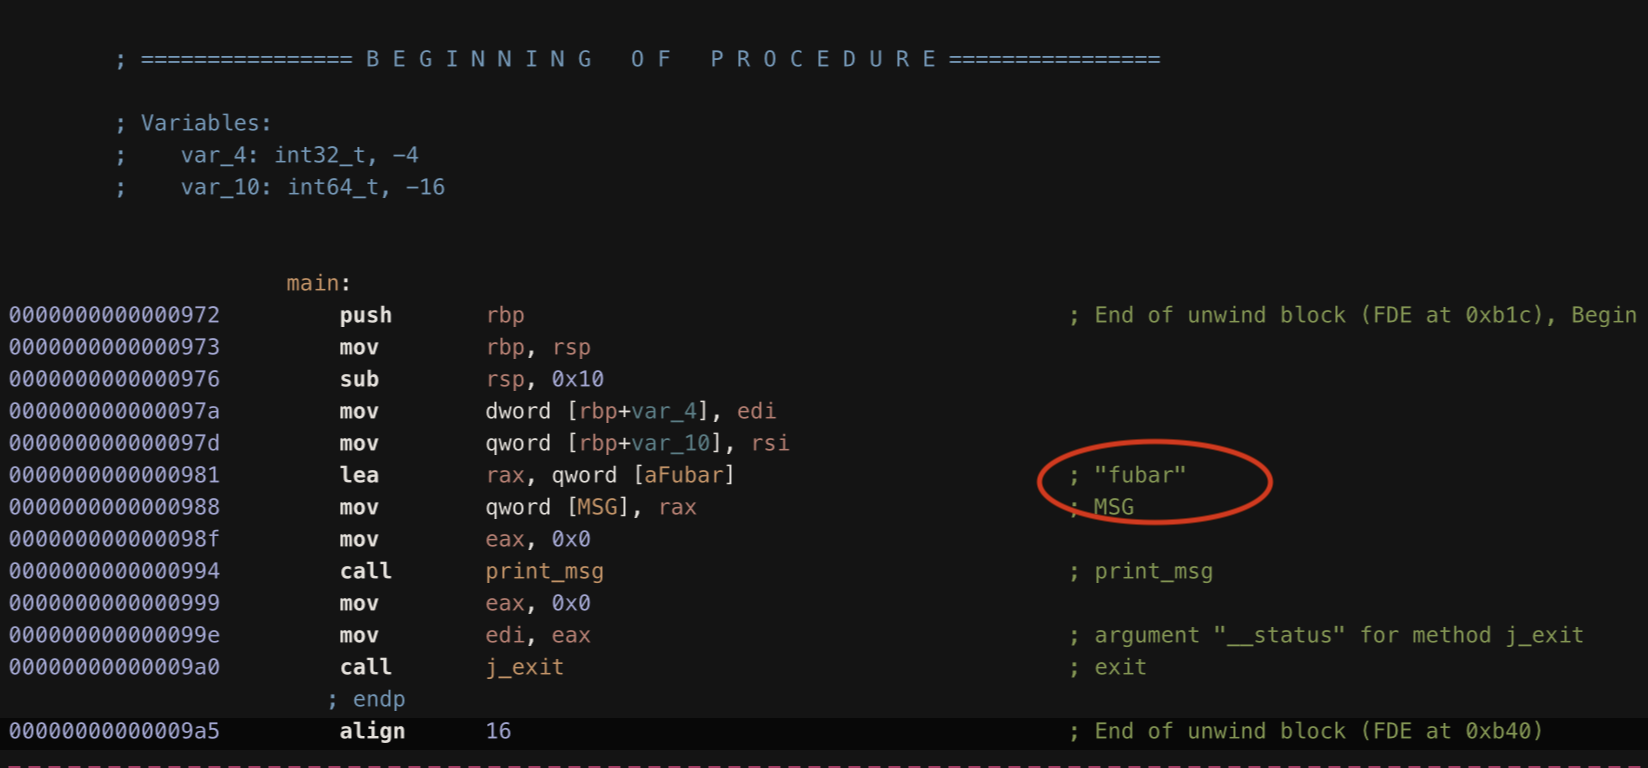
\includegraphics[width=\textwidth]{figure01.png}
%     \caption{Login Screen for Ubuntu VM.}
%     \label{fig:login}
% \end{figure}

% \begin{figure}[!ht]
%     \centering
%     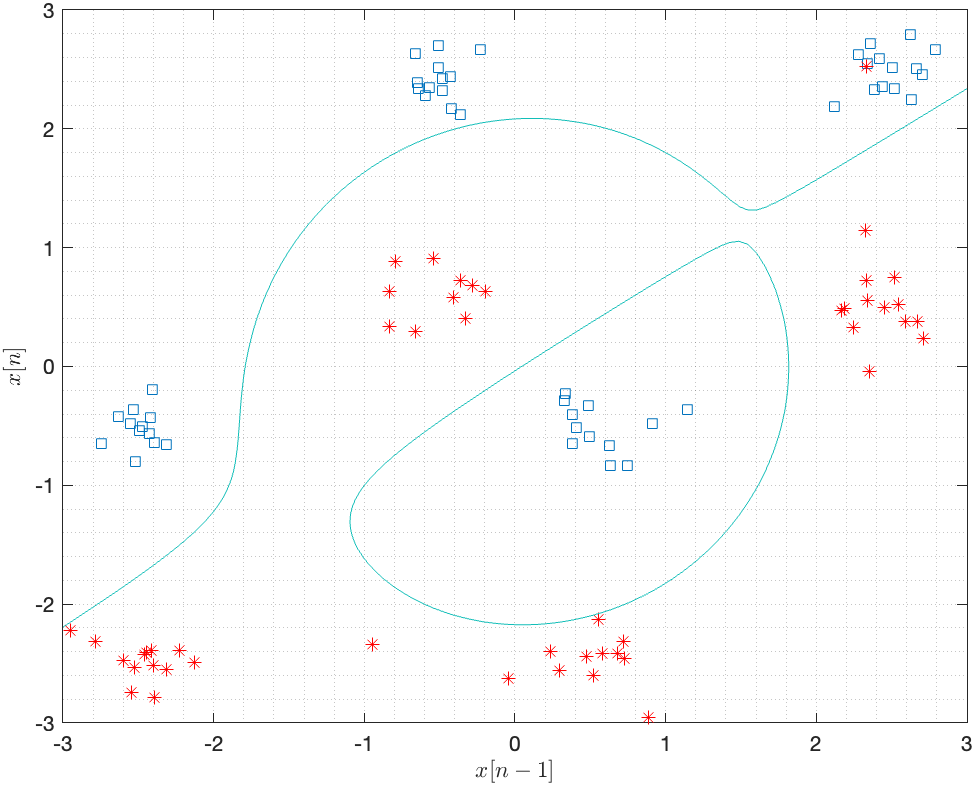
\includegraphics[width=\textwidth]{figure02.png}\vspace{-1em}
%     \caption{Settings for Ubuntu VM.}
%     \label{fig:settings}
% \end{figure}


\end{document}